\chapter{الرنين المغناطيسي النووي بعمق: النبضات والاسترخاء والأطياف الثنائية البعد}\label{ch:b3:advanced-nmr}

يعمل ماسح التصوير بالرنين المغناطيسي في المستشفى ومطياف الرنين المغناطيسي النووي في قسم
الكيمياء على المبدأ نفسه. فكل منهما يضع نوى الهيدروجين في مجال
مغناطيسي قوي، ويُميل مغنطتها بنبضة قصيرة من الأمواج الراديوية، ثم
يصغي إلى الإشارة الخافتة التي تحرّضها وهي تمور وتسترخي. فيحوّل
الماسح الإشارة إلى صورة للأنسجة الرخوة؛ ويحوّلها المطياف إلى
قائمة من الانزياحات الكيميائية والاقترانات، وبعدة نبضات متتالية،
إلى خرائط ثنائية البعد تبيّن أي ذرة ترتبط بأيها. يشرح هذا
الفصل ما تفعله النبضات، ولماذا تخبو الإشارة، وكيف تُقرأ
الأطياف الثنائية البعد --- وهي الطريقة التي تُحل بها اليوم معظم
البنى العضوية الجديدة.

\begin{recall}
فسّر مجلد السنة الأولى أطياف الرنين المغناطيسي النووي \babelsublr{${}^1$H}: الانزياح الكيميائي، والحجب،
والبروتونات المتكافئة، والتكامل، واقتران سبين--سبين، وثوابت الاقتران
والمتعددات. وأضاف مجلد السنة الثانية الرنين المغناطيسي النووي \babelsublr{${}^{13}$C} مع نزع الاقتران العريض النطاق
وDEPT، الذي أخذ تتابع نبضاته معطًى؛ وتُشرح النبضات هنا.
وعامل \cref{ch:b3:many-electron-atoms} السبين بوصفه كمية حركة زاوية. ومن
الفيزياء: للعزم المغناطيسي في مجال طاقة $-\boldsymbol\mu\cdot\mathbf B$، 
وإشغالات المستويات تتبع عامل بولتزمان $\eu^{-\Delta E/kT}$، المطوَّر
في \cref{ch:b3:partition-functions}.
\end{recall}

\begin{omfigure}
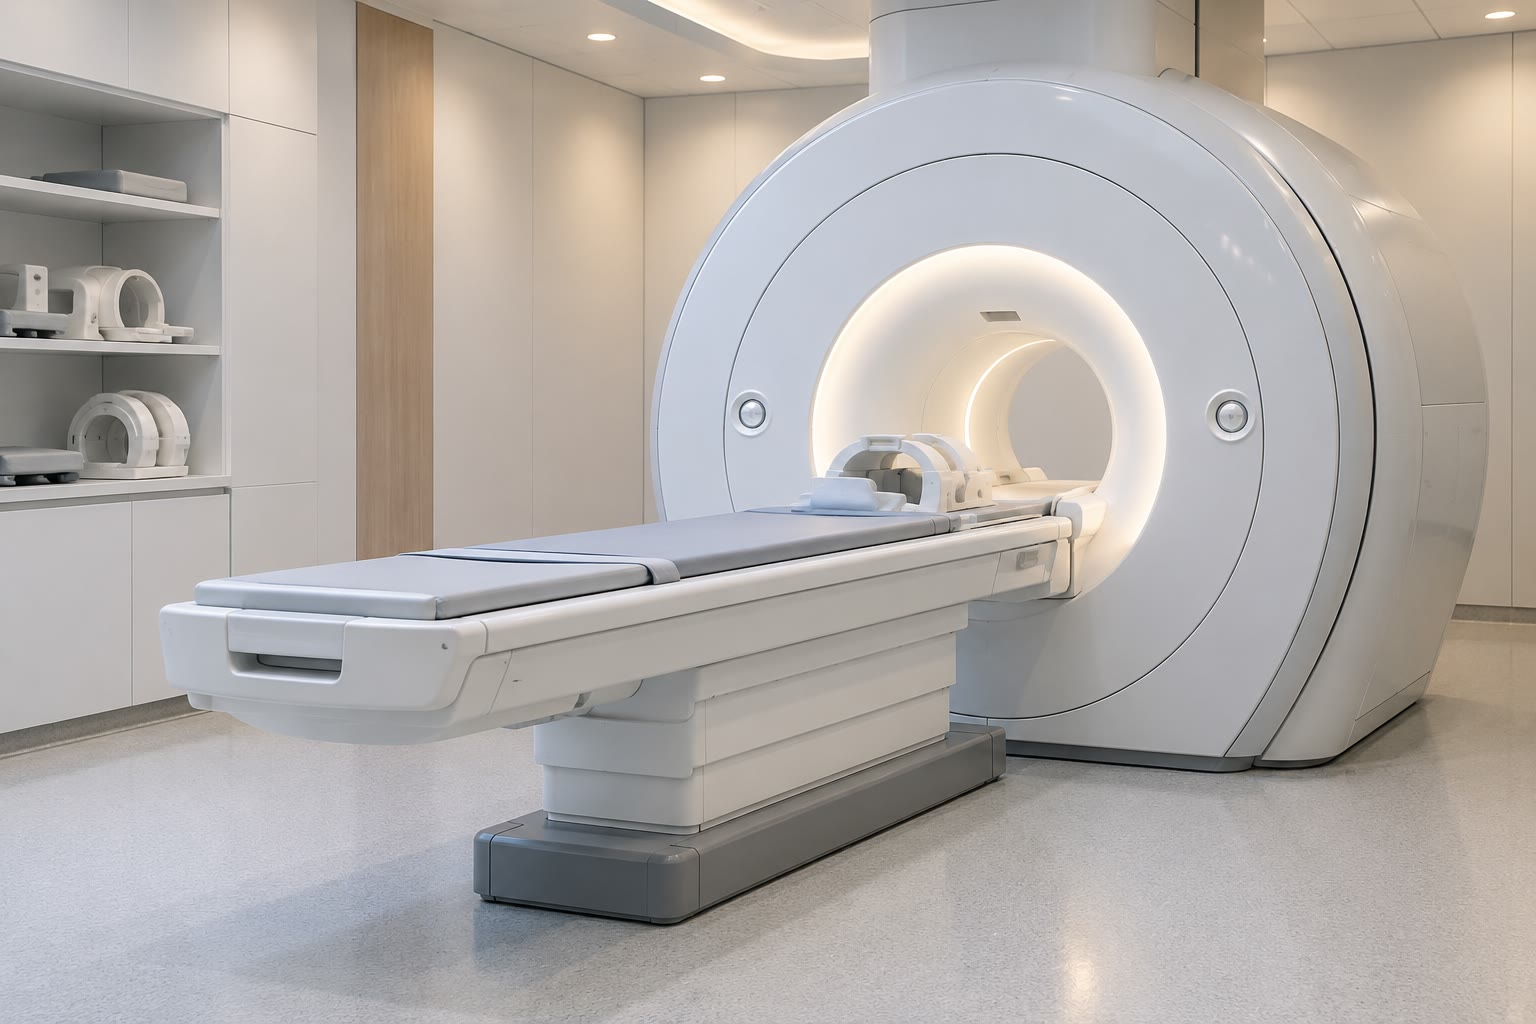
\includegraphics[width=0.52\linewidth]{images/book4/ai/b3-08-mri.jpg}\hspace{0.8em}%
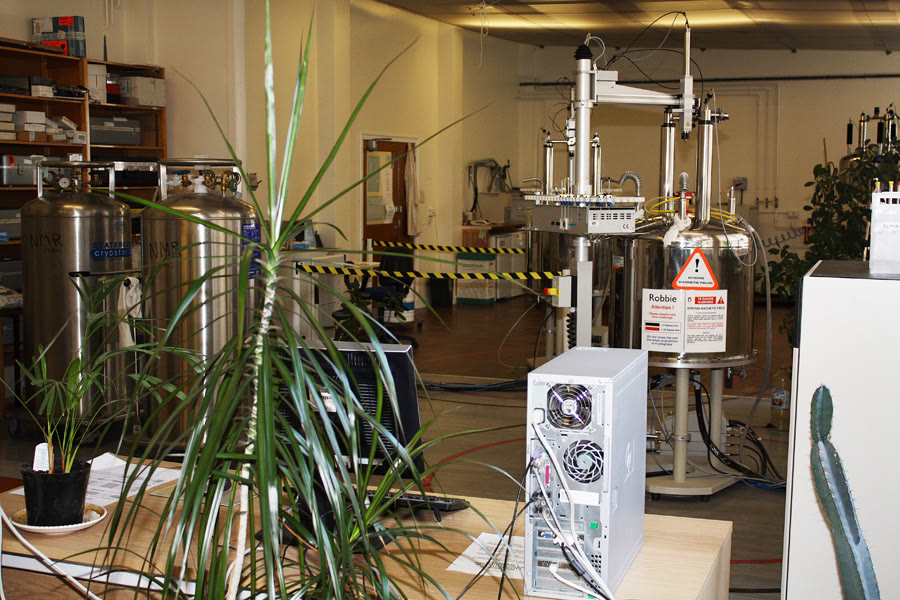
\includegraphics[width=0.4\linewidth]{images/book4/nmr-lab.jpg}

{\small يسارًا: ماسح تصوير بالرنين المغناطيسي في مستشفى. يمينًا: مختبر للرنين المغناطيسي النووي؛ كل
مغناطيس فائق الناقلية قائم في مبرّده، الذي يُعاد ملؤه بالهيليوم السائل
والنيتروجين السائل من الأوعية الحافظة على اليسار. الصورة: Shandchem،
CC BY 2.0.}
\end{omfigure}

\section{سبينات النوى في مجال مغناطيسي}

\begin{definition}[العدد الكمي لسبين النواة، النسبة الجيرومغناطيسية]\label{def:b3:advanced-nmr:nuclear-spin}
للنواة كمية حركة زاوية سبينية عددها الكمي $I$، وهو
\emph{العدد الكمي لسبين النواة}\index{العدد الكمي لسبين النواة} ($I = 0$
من أجل \ce{^{12}C} و\ce{^{16}O}؛ و$\frac12$ من أجل \ce{^1H} و\ce{^{13}C} و\ce{^{15}N} و\ce{^{19}F}
و\ce{^{31}P}؛ و1 من أجل \ce{^2H} و\ce{^{14}N})، ولها عزم مغناطيسي $\boldsymbol\mu = \gamma\hat{\mathbf
I}$ متناسب معها؛ والمقدار $\gamma$ هو \emph{النسبة الجيرومغناطيسية}\index{نسبة جيرومغناطيسية}.
وعلى امتداد مجال $B_0$ (المحور $z$)، يأخذ $\hat I_z$ القيم $m_I\hbar$،
حيث $m_I = -I, \dots, I$.
\end{definition}

\begin{proposition}[مستويات زيمان]\label{prop:b3:advanced-nmr:zeeman}
في مجال $B_0$ تكون المستويات $E_m = -m_I\gamma\hbar B_0$؛ وتمتص الانتقالات $\Delta m_I = \pm1$
عند التردد
\[
\nu_0 = \frac{\gamma B_0}{2\pi}.
\]
\end{proposition}

\begin{proof}
$E = -\boldsymbol\mu\cdot\mathbf B = -\gamma B_0\hat I_z$، وقيمه الذاتية $-\gamma B_0m_I\hbar$. والمستويان
المتجاوران يختلفان بمقدار $\gamma\hbar B_0 = h\nu_0$.
\end{proof}

\begin{definition}[تردد لارمور]\label{def:b3:advanced-nmr:larmor}
$\nu_0 = \gamma B_0/2\pi$ هو \emph{تردد لارمور}\index{تردد لارمور}
للنواة: تردد الرنين، وهو أيضًا التردد الذي يمور به عزمها
المغناطيسي حول المجال.
\end{definition}

\begin{example}[النوى الشائعة]\label{ex:b3:advanced-nmr:nuclei}
% ledger: const:gammaP, nuc:C13.mu, nuc:F19.mu, nuc:P31.mu, nuc:N15.mu, const:muN
من أجل نواة سبينها $\frac12$ وعزمها $\mu$، $\gamma/2\pi = \mu/(Ih) = 2\mu/h$. وبالعزوم
المقيسة: \ce{^1H} \qty{42.58}{MHz/T}، و\ce{^{19}F} \qty{40.08}{MHz/T}، و\ce{^{31}P}
\qty{17.25}{MHz/T}، و\ce{^{13}C} \qty{10.71}{MHz/T}، و\ce{^{15}N} \qty{-4.32}{MHz/T}. 
و«مطياف \qty{400}{MHz}» مجاله $B_0 = \qty{9.4}{T}$: فبروتوناته ترن عند
\qty{400.2}{MHz}، وذرات كربونه عند \qty{100.7}{MHz}.
\end{example}

\begin{proposition}[فرق إشغال ضئيل]\label{prop:b3:advanced-nmr:populations}
من أجل سبين $\frac12$ عند درجة الحرارة $T$، تكون زيادة عدد النوى في المستوى الأدنى
\[
\frac{N_\alpha - N_\beta}{N} \approx \frac{\gamma\hbar B_0}{2kT}.
\]
\end{proposition}

\begin{proof}
$N_\beta/N_\alpha = \eu^{-\Delta E/kT} \approx 1 - \Delta E/kT$ لأن $\Delta E \ll kT$؛ ومنه
$(N_\alpha - N_\beta)/(N_\alpha + N_\beta) \approx \Delta E/2kT$، مع $\Delta E = \gamma\hbar B_0$.
\end{proof}

من أجل البروتونات عند \qty{9.4}{T} و\qty{300}{K} تكون الزيادة \num{3.2e-5}: فلا
يساهم إلا ثلاث نوى من كل مئة ألف. وبما أن الزيادة 
والجهد المحرَّض في الملف يكبران كلاهما مع $\gamma$ و$B_0$، تكبر الإشارة
تقريبًا كالمقدار $\gamma^3B_0^2$: وهذا سبب السعي إلى مغانط أقوى فأقوى، وسبب ضعف
حساسية النوى ذات $\gamma$ الصغيرة والوفرة الطبيعية المنخفضة مثل
\ce{^{13}C}.

\section{النبضات وتناقص الحث الحر}

\begin{definition}[المغنطة الصافية، المعلم الدوّار]\label{def:b3:advanced-nmr:magnetisation}
\emph{المغنطة الصافية}\index{مغنطة صافية} $\mathbf M$ لعيّنة هي
مجموع عزومها المغناطيسية النووية في وحدة الحجم؛ وهي عند التوازن
$M_0$ على امتداد $\mathbf B_0$. و\emph{المعلم الدوّار}\index{معلم دوّار} مجموعة
محاور $x'$ و$y'$ و$z$ تدور حول $z$ بتردد الأمواج الراديوية
المطبَّقة؛ وفيه تُرى الحركة الموَرانية بالتردد $\nu_0$ مبطَّأة إلى الإزاحة $\nu_0 -
\nu_{\mathrm{rf}}$.
\end{definition}

\begin{proposition}[الحركة الموَرانية]\label{prop:b3:advanced-nmr:precession}
المغنطة في مجال تحقق $\dd\mathbf M/\dd t = \gamma\,\mathbf M\times\mathbf B$؛ وفي
مجال ساكن $B_0\mathbf e_z$، تدور مركبتها العرضية حول $z$ بالتردد
الزاوي $\omega_0 = \gamma B_0$ بينما تبقى $M_z$ ثابتة.
\end{proposition}

\begin{proof}[برهان جزئي]
المعادلة هي معادلة العزم الكلاسيكية لعزم مغناطيسي يحمل
كمية حركة زاوية، مأخوذة من الفيزياء. ومع $\mathbf B = B_0\mathbf e_z$: $\dot M_x = \gamma
B_0M_y$، $\dot M_y = -\gamma B_0M_x$، $\dot M_z = 0$، وحلها $M_x + \iu M_y \propto
\eu^{-\iu\gamma B_0t}$: دوران بالتردد $\omega_0$ (باتجاه عقارب الساعة منظورًا إليه من $+z$ من أجل $\gamma > 0$).
\end{proof}

\begin{definition}[النبضة الراديوية، زاوية القلب]\label{def:b3:advanced-nmr:pulse}
\emph{النبضة الراديوية}\index{نبضة راديوية} دفقة قصيرة من
الأمواج الراديوية بالتردد $\nu_{\mathrm{rf}} \approx \nu_0$، مجالها المغناطيسي $B_1$، الثابت في
\omterm{def:b3:advanced-nmr:magnetisation}{المعلم الدوّار} على امتداد $x'$، يُدير $\mathbf M$ حول $x'$. وزاوية الدوران هي
\emph{زاوية القلب}\index{زاوية القلب} $\theta = \gamma B_1t_p$ لنبضة مدتها
$t_p$: فالنبضة $90^\circ$ تنقل $\mathbf M$ إلى المستوي $x'y'$، والنبضة $180^\circ$ تقلبها
رأسًا على عقب.
\end{definition}

\begin{omfigure}
\tdplotsetmaincoords{70}{120}
\begin{tikzpicture}[tdplot_main_coords, font=\small, >=Stealth]
  \begin{scope}
    \draw[->, gray] (0,0,0) -- (1.8,0,0) node[anchor=north east] {$x'$};
    \draw[->, gray] (0,0,0) -- (0,1.8,0) node[anchor=north west] {$y'$};
    \draw[->, gray] (0,0,0) -- (0,0,1.8) node[anchor=south] {$z$, $\mathbf B_0$};
    \draw[->, omThm, very thick] (0,0,0) -- (0,0,1.4) node[anchor=west] {$\mathbf M$};
    \node[anchor=north] at (0,0,-0.9) {\foreignlanguage{arabic}{التوازن}};
  \end{scope}
  \begin{scope}[shift={(0,4.6,0)}]
    \draw[->, gray] (0,0,0) -- (1.8,0,0) node[anchor=north east] {$x'$};
    \draw[->, gray] (0,0,0) -- (0,1.8,0) node[anchor=north west] {$y'$};
    \draw[->, gray] (0,0,0) -- (0,0,1.8) node[anchor=south] {$z$};
    \draw[->, omDef, thick] (0,0,0) -- (1.2,0,0) node[anchor=south east, xshift=-2pt] {$\mathbf B_1$};
    \draw[->, omThm, very thick] (0,0,0) -- (0,1.4,0) node[anchor=south west] {$\mathbf M$};
    \node[anchor=north] at (0,0,-0.9) {\foreignlanguage{arabic}{بعد نبضة $90^\circ_{x'}$}};
  \end{scope}
  \begin{scope}[shift={(0,9.2,0)}]
    \draw[->, gray] (0,0,0) -- (1.8,0,0) node[anchor=north east] {$x'$};
    \draw[->, gray] (0,0,0) -- (0,1.8,0) node[anchor=north west] {$y'$};
    \draw[->, gray] (0,0,0) -- (0,0,1.8) node[anchor=south] {$z$};
    \draw[->, omThm, very thick] (0,0,0) -- (0,0,-1.4) node[anchor=west] {$\mathbf M$};
    \node[anchor=north] at (0,0,-1.6) {\foreignlanguage{arabic}{بعد نبضة $180^\circ_{x'}$}};
  \end{scope}
\end{tikzpicture}

{\small المغنطة في \omterm{def:b3:advanced-nmr:magnetisation}{المعلم الدوّار}. النبضة $90^\circ$ حول $x'$
تُدير $\mathbf M$ من $z$ إلى $y'$ (مع $\gamma > 0$ يتبع الدوران
قاعدة اليد اليسرى حول $\mathbf B_1$، وهو الاصطلاح المعتاد)؛ والنبضة $180^\circ$
تقلبها.}
\end{omfigure}

\begin{definition}[تناقص الحث الحر]\label{def:b3:advanced-nmr:fid}
بعد نبضة $90^\circ$، تمور المغنطة العرضية \omterm{def:b3:advanced-nmr:larmor}{بتردد لارمور}
وتحرّض جهدًا متذبذبًا في الملف المحيط بالعيّنة،
يخبو مع استرخاء المغنطة: وهذا \emph{تناقص الحث
الحر}\index{تناقص الحث الحر} (FID).
\end{definition}

\begin{theorem}[من FID إلى الطيف]\label{thm:b3:advanced-nmr:lorentzian}
تحويل فورييه لتذبذب متخامد $\eu^{-t/T_2}\cos(2\pi\nu t)$ ($t \ge 0$) هو،
قرب $\nu$، خط لورنتزي عرضه الكامل عند منتصف الارتفاع $1/(\pi T_2)$.
\end{theorem}

\begin{proof}
لنكتب الإشارة $\eu^{-t/T_2}\eu^{2\pi\iu\nu t}$ ولنكامل:
$\int_0^\infty\eu^{-t/T_2}\eu^{2\pi\iu(\nu - f)t}\dd t = \frac{1}{1/T_2 - 2\pi\iu(\nu - f)}$، وجزؤه
الحقيقي $\frac{T_2}{1 + 4\pi^2T_2^2(f - \nu)^2}$. وهو أعظمي عند $f = \nu$ وينخفض إلى
النصف حين $2\pi T_2|f - \nu| = 1$، أي عند $f - \nu = \pm1/(2\pi T_2)$: فالعرض الكامل
$1/(\pi T_2)$.
\end{proof}

\begin{omfigure}
\begin{tikzpicture}
\begin{axis}[name=fid, width=0.5\linewidth, height=4.6cm, xmin=0, xmax=0.4,
  ymin=-2.1, ymax=2.1, axis lines=left, xlabel={\babelsublr{$t$ / s}}, ylabel={\foreignlanguage{arabic}{الإشارة}},
  ytick=\empty, scaled x ticks=false, xticklabel style={/pgf/number format/fixed},
  tick label style={font=\small}, label style={font=\small}, title={\small \babelsublr{FID}}]
\addplot[omDef] table[x=t, y=s] {figdata/out/bachelor-3-nmr-fid.dat};
\addplot[gray, dashed, domain=0:0.4, samples=60] {2*exp(-x/0.1)};
\end{axis}
\begin{axis}[at={(fid.east)}, anchor=west, xshift=1.2cm, width=0.45\linewidth,
  height=4.6cm, xmin=0, xmax=350, ymin=-0.1, ymax=1.1, axis x line=bottom,
  axis y line=none, xlabel={\foreignlanguage{arabic}{الإزاحة الترددية \babelsublr{(Hz)}}}, tick label style={font=\small},
  label style={font=\small}, title={\small \foreignlanguage{arabic}{الطيف بعد تحويل فورييه}}]
\addplot[omThm, thick] table[x=f, y=I] {figdata/out/bachelor-3-nmr-fid-spectrum.dat};
\end{axis}
\end{tikzpicture}

{\small يسارًا: FID لخطين (إزاحتاهما 100 و\qty{250}{Hz}، $T_2 = \qty{0.10}{s}$)،
يتضاربان إذ يتداخل الترددان داخل غلاف أسي
(متقطع). يمينًا: تحويل فورييه له، خطان لورنتزيان عرض كل منهما \qty{3.2}{Hz}.}
\end{omfigure}

\begin{proposition}[متوسط الإشارات]\label{prop:b3:advanced-nmr:averaging}
جمع $N$ تسجيلًا من FID يضرب الإشارة في $N$ والضجيج العشوائي في $\sqrt N$:
فتكبر نسبة الإشارة إلى الضجيج كالمقدار $\sqrt N$.
\end{proposition}

\begin{proof}
تتجمع الإشارة تجمعًا متطاورًا. أما ضجيج التسجيلات المستقلة فمتوسطه
صفر وتباينه $\sigma^2$ في كل منها؛ وتباين مجموع $N$ حدًا مستقلًا هو
$N\sigma^2$ (قانون الانتشار في مجلد السنة الثانية)، فانحرافه المعياري
$\sqrt N\sigma$.
\end{proof}

يطبّق DEPT، الذي يفرز إشارات \babelsublr{${}^{13}$C} بحسب عدد ذرات الهيدروجين المرتبطة،
تتابعًا من النبضات على البروتونات وذرات الكربون معًا تفصل بينها
فترات انتظار قدرها $1/2J$: فتُنقل مغنطة البروتونات الكبيرة إلى الكربون
عبر الاقتران بروابط واحدة، وهذا يضاعف إشارة الكربون بعامل يقارب
$\gamma_H/\gamma_C \approx 4$، وتُرجِّح زاوية نبضة البروتون الأخيرة المجموعات CH و\ce{CH2} 
و\ce{CH3} ترجيحًا مختلفًا. والفكرة نفسها --- نقل المغنطة بين النوى
عبر اقتراناتها --- هي أساس التجارب الثنائية البعد أدناه.

\section{الاسترخاء}

\begin{definition}[زمنا الاسترخاء الطولي والعرضي]\label{def:b3:advanced-nmr:relaxation}
عودة $M_z$ إلى $M_0$ بعد اضطراب ما أسية، يحكمها
\emph{زمن الاسترخاء الطولي}\index{زمن الاسترخاء الطولي} $T_1$
(استرخاء سبين--شبكة: طاقة تُعطى للمحيط). وتناقص
المغنطة العرضية إلى الصفر أسي يحكمه
\emph{زمن الاسترخاء العرضي}\index{زمن الاسترخاء العرضي} $T_2 \le T_1$
(استرخاء سبين--سبين: فقدان الترابط الطوري بين السبينات).
\end{definition}

\begin{proposition}[الاسترداد بعد الانقلاب]\label{prop:b3:advanced-nmr:inversion-recovery}
بعد نبضة $180^\circ$، $M_z(t) = M_0(1 - 2\eu^{-t/T_1})$؛ وهي تمر بالصفر عند
$t_{\mathrm{null}} = T_1\ln2$.
\end{proposition}

\begin{proof}
لمعادلة الاسترخاء $\dd M_z/\dd t = (M_0 - M_z)/T_1$ مع $M_z(0) = -M_0$
الحل $M_0 - 2M_0\eu^{-t/T_1}$، الذي ينعدم حين $\eu^{-t/T_1} = \frac12$.
\end{proof}

\begin{method}[قياس $T_1$ وضبط فترة تكرار كمية]\label{met:b3:advanced-nmr:t1}
\begin{enumerate}
  \item نفّذ التتابع \babelsublr{$180^\circ$--$\tau$--$90^\circ$}--اقتناء من أجل سلسلة من فترات الانتظار
        $\tau$، مع انتظار $5T_1$ على الأقل بين المسوح.
  \item اضبط كل إشارة على $M_0(1 - 2\eu^{-\tau/T_1})$، أو اقرأ نقطة الانعدام: $T_1 =
        t_{\mathrm{null}}/\ln2$.
  \item من أجل تكامل كمي بنبضات $90^\circ$، انتظر بين المسوح $5T_1$ على الأقل لأبطأ
        نواة: فيكون الناقص من المغنطة عندئذ $\eu^{-5} < 1\,\%$
        فقط.
\end{enumerate}
\end{method}

\begin{omfigure}
\begin{tikzpicture}
\begin{axis}[width=0.62\linewidth, height=5cm, xmin=0, xmax=10, ymin=-1.1, ymax=1.15,
  axis lines=left, xlabel={\babelsublr{$t$ / s}}, ylabel={$M/M_0$}, legend cell align=left,
  legend style={font=\small, draw=none, at={(0.97,0.05)}, anchor=south east},
  tick label style={font=\small}, label style={font=\small}]
\addplot[omDef, thick] table[x=t, y=mz] {figdata/out/bachelor-3-nmr-relaxation.dat};
\addlegendentry{\foreignlanguage{arabic}{$M_z$ بعد $180^\circ$، \babelsublr{$T_1 = \qty{2.0}{s}$}}}
\addplot[omThm, thick, dashed] table[x=t, y=mxy] {figdata/out/bachelor-3-nmr-relaxation.dat};
\addlegendentry{\foreignlanguage{arabic}{$M_{xy}$ بعد $90^\circ$، \babelsublr{$T_2 = \qty{0.5}{s}$}}}
\addplot[gray, dotted, domain=0:10] {0};
\addplot[only marks, mark=*, mark size=1.5pt, black] coordinates {(1.386,0)};
\node[font=\small, anchor=north west] at (axis cs:1.5,-0.04) {$T_1\ln2$};
\end{axis}
\end{tikzpicture}

{\small الاسترخاء (قيم نموذجية). تعود المغنطة الطولية المقلوبة
مارةً بالصفر عند $T_1\ln2$؛ وتتناقص المغنطة العرضية
أسرع، بالزمن $T_2$.}
\end{omfigure}

\begin{definition}[صدى السبين]\label{def:b3:advanced-nmr:echo}
في التتابع \babelsublr{$90^\circ$--$\tau$--$180^\circ$--$\tau$}، تُعاد السبينات التي تباعدت أطوارها
بسبب عدم تجانس المجال إلى التطاور عند الزمن $2\tau$، فينشأ
\emph{صدى السبين}\index{صدى السبين}؛ وتتناقص سعته بالزمن $T_2$ الحقيقي، متحررةً من
عدم تجانس المغناطيس.
\end{definition}

\begin{definition}[مفعول أوفرهاوزر النووي]\label{def:b3:advanced-nmr:noe}
إشباع سبين ما أو اضطرابه يغيّر، عبر استرخائهما
ثنائي القطب، شدة إشارة سبين آخر قريب منه في الفضاء:
وهذا \emph{مفعول أوفرهاوزر النووي}\index{مفعول أوفرهاوزر النووي} (NOE).
وسرعة نشوئه متناسبة مع $r^{-6}$، فلا يُرى إلا بين
نوى يفصل بينها أقل من نحو \qty{0.5}{nm}، مترابطة كانت أم لا.
\end{definition}

\section{الرنين المغناطيسي النووي الثنائي البعد}

\begin{definition}[الطيف الثنائي البعد، القمة المتقاطعة، القمة القطرية]\label{def:b3:advanced-nmr:two-d}
\emph{الطيف الثنائي البعد}\index{طيف ثنائي البعد} يُسجَّل
بتكرار تتابع نبضات مع زيادة فترة الانتظار $t_1$ قبل
زمن الاقتناء $t_2$؛ ويعطي تحويل فورييه المزدوج خريطة للشدة
بدلالة ترددين. و\emph{القمة المتقاطعة}\index{قمة متقاطعة} عند $(\delta_1,
\delta_2)$ تبيّن أن النواتين عند $\delta_1$ و$\delta_2$ متصلتان (باقتران أو
بقرب)؛ و\emph{القمة القطرية}\index{قمة قطرية} عند $(\delta, \delta)$ تخص
نواة واحدة.
\end{definition}

\begin{definition}[COSY، HSQC، HMBC، NOESY]\label{def:b3:advanced-nmr:experiments}
\emph{COSY}\index{COSY} (مطيافية الارتباط) تربط بين البروتونات المقترنة
بعضها ببعض، عادة عبر ثلاث روابط (H--C--C--H). و\emph{HSQC}\index{HSQC}
(ترابط التماسك الأحادي الكم غير المتجانس النوى) تربط كل ذرة كربون بالبروتونات
المرتبطة بها مباشرة. و\emph{HMBC}\index{HMBC} (الترابط غير المتجانس النوى
عبر روابط متعددة) تربط ذرات الكربون بالبروتونات البعيدة عنها رابطتين أو ثلاثًا،
عبر ذرات الكربون الرباعية والذرات المغايرة. و\emph{NOESY}\index{NOESY}
تربط البروتونات المتقاربة في الفضاء عبر \omterm{def:b3:advanced-nmr:noe}{مفعول أوفرهاوزر النووي}.
\end{definition}

\begin{omfigure}
\begin{tikzpicture}[font=\small]
  \foreach \y/\name in {3.2/{\foreignlanguage{arabic}{نبضة واحدة}}, 2.0/{\foreignlanguage{arabic}{استرداد بعد الانقلاب}}, 0.8/{\foreignlanguage{arabic}{صدى السبين}}, -0.4/{COSY}}{
    \draw (0,\y) -- (9.3,\y); \node[anchor=east] at (-0.1,\y+0.25) {\name};}
  % one pulse
  \fill[black] (0.4,3.2) rectangle (0.6,3.75);
  \draw[omDef, domain=0:3.5, samples=120] plot (0.7+\x, {3.2+0.4*exp(-\x/1.2)*sin(\x*500)});
  % inversion recovery
  \fill[black] (0.4,2.0) rectangle (0.8,2.55); \node[font=\scriptsize] at (0.6,2.7) {180};
  \draw[<->] (0.85,1.85) -- (2.4,1.85) node[midway, below, font=\scriptsize] {$\tau$};
  \fill[black] (2.45,2.0) rectangle (2.65,2.55); \node[font=\scriptsize] at (2.55,2.7) {90};
  \draw[omDef, domain=0:3.0, samples=120] plot (2.75+\x, {2.0+0.4*exp(-\x/1.0)*sin(\x*500)});
  % spin echo
  \fill[black] (0.4,0.8) rectangle (0.6,1.35); \node[font=\scriptsize] at (0.5,1.5) {90};
  \draw[<->] (0.65,0.65) -- (2.4,0.65) node[midway, below, font=\scriptsize] {$\tau$};
  \fill[black] (2.45,0.8) rectangle (2.85,1.35); \node[font=\scriptsize] at (2.65,1.5) {180};
  \draw[<->] (2.9,0.65) -- (4.65,0.65) node[midway, below, font=\scriptsize] {$\tau$};
  \draw[omDef, domain=-1.2:2.5, samples=150] plot (4.65+\x, {0.8+0.35*exp(-abs(\x)/0.35)*cos(\x*700)});
  % COSY
  \fill[black] (0.4,-0.4) rectangle (0.6,0.15); \node[font=\scriptsize] at (0.5,0.3) {90};
  \draw[<->] (0.65,-0.55) -- (2.4,-0.55) node[midway, below, font=\scriptsize] {\foreignlanguage{arabic}{$t_1$ متزايد}};
  \fill[black] (2.45,-0.4) rectangle (2.65,0.15); \node[font=\scriptsize] at (2.55,0.3) {90};
  \draw[omDef, domain=0:3.0, samples=120] plot (2.75+\x, {-0.4+0.4*exp(-\x/1.0)*sin(\x*500)});
  \node[font=\scriptsize, anchor=west] at (5.9,-0.2) {\foreignlanguage{arabic}{الاقتناء $t_2$}};
\end{tikzpicture}

{\small تتابعات النبضات (الزمن نحو اليمين؛ المستطيلات الممتلئة: نبضات، موسومة
\omterm{def:b3:advanced-nmr:pulse}{بزوايا قلبها} بالدرجات؛ والأزرق: الإشارة المسجلة). يبلغ \omterm{def:b3:advanced-nmr:echo}{صدى السبين}
ذروته عند $2\tau$ بعد النبضة الأولى.}
\end{omfigure}

\begin{method}[حل بنية بالأطياف الثنائية البعد]\label{met:b3:advanced-nmr:solve-2d}
\begin{enumerate}
  \item من الصيغة، وتكاملات \babelsublr{${}^1$H} وطيف \babelsublr{${}^{13}$C}/DEPT، اكتب قائمة
        ذرات الكربون CH و\ce{CH2} و\ce{CH3} والرباعية.
  \item \omterm{def:b3:advanced-nmr:experiments}{HSQC}: اربط كل إشارة بروتون بذرة كربونها.
  \item \omterm{def:b3:advanced-nmr:experiments}{COSY}: اجمع ذرات الكربون المحمولة على بروتونات في أنظمة سبينية (سلاسل من
        الجيران).
  \item \omterm{def:b3:advanced-nmr:experiments}{HMBC}: اربط الأنظمة السبينية عبر ذرات الكربون الرباعية والكربونيلات 
        والذرات المغايرة، حيث يصمت \omterm{def:b3:advanced-nmr:experiments}{COSY}.
  \item \omterm{def:b3:advanced-nmr:experiments}{NOESY}: عيّن الترتيبات الفراغية النسبية والتشكلات من
        التماسات عبر الفضاء.
  \item تحقق من كل إشارة مقابل البنية المقترحة.
\end{enumerate}
\end{method}

\begin{omfigure}
\begin{tikzpicture}
\begin{axis}[name=cosy, width=0.47\linewidth, height=0.47\linewidth, x dir=reverse,
  y dir=reverse, xmin=0.5, xmax=4.6, ymin=0.5, ymax=4.6, axis lines=box,
  xlabel={\babelsublr{$\delta_{\mathrm H}$ / ppm}}, ylabel={\babelsublr{$\delta_{\mathrm H}$ / ppm}},
  tick label style={font=\small}, label style={font=\small}, title={\small \babelsublr{COSY}}]
\addplot[gray, dotted, domain=0.5:4.6] {x};
\addplot[only marks, mark=*, mark size=2.2pt, black] table[x=h1, y=h2] {figdata/out/bachelor-3-nmr-2d-cosy-diag.dat};
\addplot[only marks, mark=*, mark size=2.2pt, omThm] table[x=h1, y=h2] {figdata/out/bachelor-3-nmr-2d-cosy-cross.dat};
\end{axis}
\begin{axis}[at={(cosy.east)}, anchor=west, xshift=1.3cm, width=0.47\linewidth,
  height=0.47\linewidth, x dir=reverse, y dir=reverse, xmin=0.5, xmax=4.6,
  ymin=0, ymax=185, axis lines=box, xlabel={\babelsublr{$\delta_{\mathrm H}$ / ppm}},
  ylabel={\babelsublr{$\delta_{\mathrm C}$ / ppm}}, tick label style={font=\small},
  label style={font=\small}, title={\small \foreignlanguage{arabic}{\babelsublr{HSQC} بالأزرق و\babelsublr{HMBC} بالأحمر}}]
\addplot[only marks, mark=square*, mark size=2.2pt, omDef] table[x=h, y=c] {figdata/out/bachelor-3-nmr-2d-hsqc.dat};
\addplot[only marks, mark=o, mark size=2.6pt, omThm, thick] table[x=h, y=c] {figdata/out/bachelor-3-nmr-2d-hmbc.dat};
\end{axis}
\end{tikzpicture}

{\small الأطياف الثنائية البعد لبوتانوات الإيثيل، \ce{CH3CH2CH2COOCH2CH3}،
مرسومة عند انزياحاته المقيسة. \omterm{def:b3:advanced-nmr:experiments}{COSY}: بالأسود، القمم القطرية؛ وبالأحمر، القمم المتقاطعة
بين بروتونات على ذرات كربون متجاورة --- نظامان سبينيان، الإيثيل 
والبروبيل، دون أي \omterm{def:b3:advanced-nmr:two-d}{قمة متقاطعة} عبر أكسجين الإستر. يمينًا: قمم \omterm{def:b3:advanced-nmr:experiments}{HSQC}
(مربعات) تربط كل بروتون بكربونه؛ وقمم \omterm{def:b3:advanced-nmr:experiments}{HMBC} (دوائر) تبيّن أن بروتونات \babelsublr{OCH$_2$}
(\qty{4.13}{ppm}) وبروتونات \babelsublr{CH$_2$C}=O (\qty{2.28}{ppm}) تبلغان كلتاهما
كربون الكربونيل عند \qty{173.6}{ppm}.}
\end{omfigure}

\section{نوى أخرى والديناميكا}

الفلور-19 والفوسفور-31، وسبين كل منهما $\frac12$، ووفرتهما 100\,\% و$\gamma$
لكل منهما كبيرة، يكاد رصدهما يكون في سهولة رصد البروتونات؛ ومجالات انزياحاتهما الواسعة تجعلهما
مسبارين دقيقين لمحيطهما (الأدوية، والفوسفات، والربائط مثل
الفوسفينات في \cref{ch:b3:organometallic-bonding}). أما النيتروجين-15 فنادر 
وضعيف، ويُرصد عادة رصدًا غير مباشر عبر البروتونات المرتبطة به.
ويُزال الاقتران بين نوى مختلفة بنزع الاقتران، كما في \babelsublr{${}^{13}$C} في
مجلد السنة الثانية.

\begin{definition}[درجة حرارة الاندماج]\label{def:b3:advanced-nmr:coalescence}
حين تتبادل نواة بين بيئتين يفصل بين انزياحيهما
$\Delta\nu$ (بالهرتز)، يتعرض خطاها كلما تسارع التبادل ثم يندمجان
في خط واحد عند \emph{درجة حرارة الاندماج}\index{درجة حرارة الاندماج}
$T_c$.
\end{definition}

\begin{proposition}[السرعة عند الاندماج]\label{prop:b3:advanced-nmr:coalescence}
من أجل موقعين متساويي الإشغال دون اقتران، يكون ثابت سرعة التبادل عند
الاندماج $k_c = \pi\Delta\nu/\sqrt2$.
\end{proposition}
\admitted

يُتناول الاستنتاج، من معادلات بلوخ مع التبادل، في مقررات أكثر
تقدمًا. وبمعادلة أيرنغ (\cref{ch:b3:rate-theories}) تعطي السرعة
الحاجز: فالرنين المغناطيسي النووي الديناميكي يقيس الدوران حول روابط الأميد، وانقلاب
الحلقات وتبادل الربائط ذات الحواجز من 40 إلى \qty{100}{kJ/mol}.

\begin{example}[صورة بالرنين المغناطيسي]\label{ex:b3:advanced-nmr:mri}
في التصوير بالرنين المغناطيسي يجعل تدرّجُ المجال ترددَ لارمور
لبروتونات الماء متعلقًا بالموضع، فيكون تحويل فورييه
للإشارة خريطة لمواضعها. ويأتي التباين من الاسترخاء: فيُختار
زمن التكرار وفترات الصدى لترجيح الصورة بالزمن $T_1$ أو بالزمن
$T_2$، اللذين يختلفان من نسيج إلى آخر؛ وعوامل التباين المحتوية على الغادولينيوم
تقصّر $T_1$ للماء القريب منها (\cref{ch:b3:bioinorganic}).
\end{example}

\begin{inthelab}[تحضير المطياف]
تُنزل العيّنة، المذابة في مذيب مُدَوْتَر، في المسبار.
ويثبّت المطياف القفل على إشارة الدوتيريوم لتعويض الانحراف البطيء
للمجال؛ ويُضبط المسبار ويُوائَم على تردد كل نواة؛
ويُجعل المجال متجانسًا على العيّنة بضبط ملفات التسوية
حتى تضيق الخطوط. ومجال المغناطيس دائم: فتُبقى الأدوات الفولاذية
وبطاقات الائتمان وأجهزة تنظيم ضربات القلب خارج خط الأمان المعلَّم.
\end{inthelab}

\begin{history}[من الرنين إلى البعدين]
رصد فيليكس بلوخ وإدوارد بورسل الرنين المغناطيسي النووي في المادة
الكتلية سنة 1946 (جائزة نوبل في الفيزياء، 1952). وأدخل ريتشارد إرنست الرنين المغناطيسي النووي النبضي
بتحويل فورييه سنة 1966، ثم، اتباعًا لفكرة لجان جينر،
المطيافية الثنائية البعد في السبعينيات (جائزة نوبل في الكيمياء، 1991).
\end{history}

\section{تمارين}

\begin{exercise}[$\star$]\label{exo:b3:advanced-nmr:1}
% ledger: const:gammaP, nuc:C13.mu, nuc:F19.mu
احسب ترددات لارمور للنوى \ce{^1H} و\ce{^{13}C} و\ce{^{19}F} عند \qty{14.1}{T}
($\gamma/2\pi = 42.58$ و10.71 و\qty{40.08}{MHz/T}).
\end{exercise}

\begin{exercise}[$\star$]\label{exo:b3:advanced-nmr:2}
احسب الزيادة النسبية للبروتونات في المستوى الأدنى عند \qty{9.4}{T} 
و\qty{300}{K}. وكم تتغير عند \qty{4}{K}؟
\end{exercise}

\begin{exercise}[$\star$]\label{exo:b3:advanced-nmr:3}
تدوم نبضة $90^\circ$ مدة \qty{10}{\micro s} من أجل البروتونات. ما قيمة $\gamma B_1/2\pi$؟ وكم تدوم
نبضة $180^\circ$، وماذا تفعل نبضة مدتها \qty{5}{\micro s}؟
\end{exercise}

\begin{exercise}[$\star$]\label{exo:b3:advanced-nmr:4}
عرض خط عند منتصف ارتفاعه \qty{3.2}{Hz}. ما قيمة $T_2$ (بافتراض مجال
متجانس تمامًا)؟
\end{exercise}

\begin{exercise}[$\star\star$]\label{exo:b3:advanced-nmr:5}
% ledger: iso:C13
باستعمال إشارة $\propto\gamma^3$ لكل نواة والوفرة الطبيعية 1.1\,\% للنظير
\ce{^{13}C}، قارن حساسية الرنين المغناطيسي النووي \babelsublr{${}^{13}$C} و\babelsublr{${}^1$H}. كم مسحًا إضافيًا
يحتاج طيف \babelsublr{${}^{13}$C} للحصول على نسبة الإشارة إلى الضجيج نفسها؟
\end{exercise}

\begin{exercise}[$\star\star$]\label{exo:b3:advanced-nmr:6}
في تجربة استرداد بعد الانقلاب تختفي إشارة ذرة كربون عند
$\tau = \qty{1.39}{s}$. جد $T_1$ وفترة التكرار اللازمة للعمل الكمي.
\end{exercise}

\begin{exercise}[$\star\star$]\label{exo:b3:advanced-nmr:7}
في طيف \omterm{def:b3:advanced-nmr:experiments}{COSY} للبوتانون، \ce{CH3COCH2CH3}، أي القمم المتقاطعة تظهر؟
وأي ذرات الكربون تُظهر قمم \omterm{def:b3:advanced-nmr:experiments}{HMBC} انطلاقًا من بروتونات الميثيل الأحادية؟
\end{exercise}

\begin{exercise}[$\star\star$]\label{exo:b3:advanced-nmr:8}
إشارتا ميثيل لأميد، تتباعدان \qty{50}{Hz} في درجة حرارة منخفضة، تندمجان عند
\qty{330}{K}. احسب سرعة التبادل عند الاندماج وطاقة جيبس
للتنشيط بالعلاقة $\Delta G^\ddagger = RT_c\ln(k_BT_c/hk_c)$.
\end{exercise}

\begin{exercise}[$\star\star$]\label{exo:b3:advanced-nmr:9}
مفعول NOE بين البروتونين \babelsublr{H$_a$} و\babelsublr{H$_b$} أشد بأربع مرات منه بين \babelsublr{H$_a$} 
و\babelsublr{H$_c$}، اللذين يبعدان \qty{0.30}{nm}. قدّر المسافة \babelsublr{H$_a$--H$_b$}.
\end{exercise}

\begin{exercise}[$\star\star\star$]\label{exo:b3:advanced-nmr:10}
بيّن، بحل $\dd\mathbf M/\dd t = \gamma\mathbf M\times\mathbf B_1$ في \omterm{def:b3:advanced-nmr:magnetisation}{المعلم الدوّار}
مع $\mathbf B_1$ على امتداد $x'$، أن النبضة تُدير $\mathbf M$ بزاوية $\gamma B_1t_p$ حول $x'$.
\end{exercise}

\begin{exercise}[$\star\star\star$]\label{exo:b3:advanced-nmr:11}
فسّر لماذا يعيد \omterm{def:b3:advanced-nmr:echo}{صدى السبين} التطاور الضائع بسبب عدم تجانس
المجال لكن لا يعيد الضائع بسبب التآثرات العشوائية بين السبينات. وأي ثابت
زمني تقيسه سعة الصدى؟
\end{exercise}

\begin{exercise}[$\star\star\star$]\label{exo:b3:advanced-nmr:12}
اقترح بنية مركب \ce{C4H8O2} يُظهر طيفه \babelsublr{${}^1$H}
رباعيًا (2H، 4.12 ppm)، وأحاديًا (3H، 2.05 ppm)، وثلاثيًا (3H،
1.26 ppm)، ويربط طيفه \omterm{def:b3:advanced-nmr:experiments}{HMBC} بروتونات الرباعي بذرة
كربون عند 171 ppm (معطيات التمرين). وأي إستر آخر له الصيغة
نفسها يعطي نمط \omterm{def:b3:advanced-nmr:experiments}{HMBC} مختلفًا، وكيف؟
\end{exercise}

\section{مسألة: إستر الأناناس في بعدين}

\begin{problem}[{مسألة نهاية الأسبوع --- حل بنية بوتانوات الإيثيل من جديد، من
الأطياف الثنائية البعد: الأنظمة السبينية من COSY، وذرات الكربون من HSQC، 
ورابطة الإستر من HMBC، وفترة الانتظار اللازمة لطيف كربون
كمي}]
\label{pb:b3:advanced-nmr:1}
% ledger: nmr:ethylbutanoate-OCH2, nmr:ethylbutanoate-CH2CO, nmr:ethylbutanoate-CH2, nmr:ethylbutanoate-OCH2CH3, nmr:ethylbutanoate-CH3, c13:ethylbutanoate.CO, c13:ethylbutanoate.OCH2, c13:ethylbutanoate.CH2CO, c13:ethylbutanoate.CH2, c13:ethylbutanoate.OCH2CH3, c13:ethylbutanoate.CH3
يُظهر إستر \ce{C6H12O2} من رائحة الأناناس إشارات \babelsublr{${}^1$H} عند 4.13 (2H،
q)، و2.28 (2H، t)، و1.66 (2H، m)، و1.25 (3H، t) و0.95 ppm (3H، t)، وإشارات \babelsublr{${}^{13}$C}
عند 173.6 و60.1 و36.3 و18.6 و14.3 و13.7 ppm، مسجلة عند \qty{9.4}{T}. وأطيافه الثنائية
البعد هي تلك المبينة في الشكل في القسم 4. معطيات المسألة: قيم $T_1$
لذرات الكربون نحو \qty{20}{s} للكربونيل ومن 2 إلى \qty{6}{s} لبقية
الذرات.

\medskip\noindent\textbf{الجزء الأول --- بعد واحد.}
\begin{enumerate}
  \item احسب درجة عدم التشبع للمركب \ce{C6H12O2}.
  \item أي إشارة \babelsublr{${}^{13}$C} هي الكربونيل؟ وأيها الكربون المرتبط بالأكسجين؟
  \item كم ذرة كربون محمولة على بروتونات توجد؟ وماذا يُظهر DEPT-135؟
  \item عند \qty{9.4}{T}، ما \omterm{def:b3:advanced-nmr:larmor}{تردد لارمور} للنواتين \babelsublr{${}^1$H} و\babelsublr{${}^{13}$C}؟
  \item ثابت اقتران الرباعي \qty{7.2}{Hz}. كم عرض الرباعي بالجزء من المليون
        عند \qty{400}{MHz}؟
  \item لماذا قد تترك الأطياف الأحادية البعد وحدها ترتيب الشظايا مفتوحًا؟
\end{enumerate}

\medskip\noindent\textbf{الجزء الثاني --- \omterm{def:b3:advanced-nmr:experiments}{COSY}.}
\begin{enumerate}[resume]
  \item اكتب القمم المتقاطعة في خريطة \omterm{def:b3:advanced-nmr:experiments}{COSY}.
  \item استنتج النظامين السبينيين.
  \item لماذا لا توجد \omterm{def:b3:advanced-nmr:two-d}{قمة متقاطعة} بين 4.13 و2.28 ppm؟
  \item أي إشارة بروتون مقترنة بإشارتين أخريين؟ فسّر تعدديتها.
  \item ماذا كانت ستعني \omterm{def:b3:advanced-nmr:two-d}{قمة متقاطعة} بين 0.95 و1.25 ppm؟
  \item ارسم الشظيتين.
\end{enumerate}

\medskip\noindent\textbf{الجزء الثالث --- \omterm{def:b3:advanced-nmr:experiments}{HSQC} \omterm{def:b3:advanced-nmr:experiments}{وHMBC}.}
\begin{enumerate}[resume]
  \item من طيف \omterm{def:b3:advanced-nmr:experiments}{HSQC}، أسند كل ذرة كربون إلى بروتوناتها.
  \item أي ذرتي كربون ميثيل لا يميّز بينهما إلا \omterm{def:b3:advanced-nmr:experiments}{HSQC}؟
  \item أي قمة \omterm{def:b3:advanced-nmr:experiments}{HMBC} تربط شظية الإيثيل بالكربونيل، وعبر
        كم رابطة؟
  \item أي قمم \omterm{def:b3:advanced-nmr:experiments}{HMBC} تربط شظية البروبيل بالكربونيل؟
  \item استنتج البنية، واستبعد متماكبها بروبانوات البروبيل.
  \item لماذا تغيب عادة قمم \omterm{def:b3:advanced-nmr:experiments}{HMBC} عبر أربع روابط أو أكثر؟
\end{enumerate}

\medskip\noindent\textbf{الجزء الرابع --- طيف كربون كمي.}
\begin{enumerate}[resume]
  \item لماذا لا تتناسب تكاملات طيف \babelsublr{${}^{13}$C} العادي مع
        عدد ذرات الكربون؟
  \item ما نسبة مغنطة التوازن التي يستعيدها الكربونيل
        إذا كُررت المسوح كل \qty{5}{s} بنبضات $90^\circ$ (انطلاقًا في كل مرة
        من الصفر)؟
  \item وما النسبة بعد $5T_1$؟
  \item إلى جانب الاسترخاء، أي مفعول لنزع اقتران البروتونات يشوّه تكاملات
        الكربون، وكيف يُلغى؟
  \item بفترة انتظار $5T_1$، كم تستغرق 256 مسحًا؟
  \item اذكر النتيجة: أقصر فترة تكرار لطيف \babelsublr{${}^{13}$C}
        كمي لهذا الإستر.
\end{enumerate}
\end{problem}
